%******************** Pre Ambulo *********************************
\documentclass[12pt,a4paper]{article}
\usepackage[utf8]{inputenc}
\usepackage[portuguese]{babel}
\usepackage[T1]{fontenc}
\usepackage{amsmath}
\usepackage{amsfonts}
\usepackage{amssymb}
\usepackage{makeidx}
\usepackage{graphicx}
\usepackage{setspace}
\usepackage[left=2cm,right=2cm,top=2cm,bottom=2cm]{geometry}
\usepackage{xcolor}
\usepackage{indentfirst} %Identação do primeiro parágrafo

\usepackage[pdftex]{hyperref}

\usepackage{float}%this is important to align figures
% Definindo novas cores
\definecolor{verde}{rgb}{0.25,0.5,0.35}
\definecolor{jpurple}{rgb}{0.5,0,0.35}
\definecolor{jyellow}{rgb}{218,165,032}
% Configurando layout para mostrar codigos Java
\usepackage{listings}
\lstset{
  language=Java,
  basicstyle=\ttfamily\small, 
  keywordstyle=\color{blue}\bfseries,
  stringstyle=\color{verde},
  commentstyle=\color{gray},
  morecomment=[s][\color{gray}]{/**}{*/},
  extendedchars=true, 
  showspaces=false, 
  showstringspaces=false, 
  numbers=left,
  numberstyle=\tiny,
  breaklines=true, 
  backgroundcolor=\color{cyan!10}, 
  breakautoindent=true, 
  captionpos=b,
  xleftmargin=0pt,
  tabsize=4
}

\usepackage{fancyhdr}
\pagestyle{fancy}
\lhead{CMCC}
%\chead{Centro do Cabeçalho}
%\rhead{Direita do Cabeçalho}
\lfoot{UFABC}
%\cfoot{Centro do Rodapé}
\rfoot{Tutorial aplicativo Web com JAVA EE}
\renewcommand{\headrulewidth}{2pt}
\renewcommand{\footrulewidth}{2pt}
\author{Charles Henrique Porto Ferreira}
\title{Tutorial Desenvolvimento de aplicativos WEB com JAVA EE 2}
\begin{document}
\onehalfspacing 
\maketitle



%\hrulefill\\
%\begin{center}
%	\begin{minipage}{8cm}
%		\textbf{Aluno:} \textit{Charles Henrique Porto Ferreira}\\
%	\end{minipage}
%\end{center}
%\hrulefill\\

%\hrulefill
%\begin{center}
%	\textbf{Professor:} \textit{Andre Guilherme Ribeiro Balan}\\
%	\textbf{Centro}:\textit{ CMCC}\\
%\end{center}
%\hrulefill

\newpage
\tableofcontents

\newpage
\section{Introdução}

Na primeira parte do tutorial foi exemplificada uma pequena aplicação \textbf{CRUD}(Create Remove Update Destroy) usando a IDE \textit{Netbeans} com tecnologia JAVA EE. Grande parte do código foi gerada pelo \textit{Netbeans}, de forma a deixar transparente vários detalhes de programação que envolviam aquela pequena aplicação.

Este segundo tutorial terá como foco desenvolver a mesma aplicação do tutorial anterior, porém  minimizando o uso de ferramentas de geração de código. Serão usados somente recursos de ajuda mínima disponibilizados pela IDE, tais como organização dos pacotes e arquivos de metadados para configurações de baixo nível. Um outro aspecto que será abordado neste segundo tutorial é o tratamento do problema $n+1$ \textit{selects} e a adoção do \textit{framework \textbf{Hibernate}} para a solução do problema.

\newpage
\section{Problema do $n+1$ selects}
No exemplo da aplicação CRUD existe um problema de performance que pode passar despercebido devido à simplicidade daquela aplicação, mas que pode se tornar um grande agravante em uma aplicação maior. Ao clicar no \textit{link} para listar as turmas, é aberta uma página com uma tabela onde são mostradas todas as turmas com seus respectivos docentes e disciplinas associados. Para mostrar esses dados, o banco de dados deve ser acessado para retirar tais informações. O problema aparece exatamente neste momento, pois para conseguir os dados de uma turma é necessário encontrar o docente e a disciplina associados a essa turma. Sendo assim, da forma como esta implementado, o algoritmo faz um \textit{select} para buscar todas as turmas e para cada turma faz um novo \textit{select} para buscar seu docente. Se tivermos $n$ docentes totalizaremos $n+1$ \textit{selects} executados somente para buscar os docentes.

O processo de automatizar o acesso ao banco de dados pelo JPA traz inúmeras vantagens ao programador, deixando transparente vários aspectos de baixo nível na programação. Entretanto algumas otimizações feitas pelo JPA podem ajudar por um lado mas dificultar por outro. Como é o caso do problema do $n+1$ selects. A solução adotada para resolver esse problema foi usar o framework do Hibernate que fornece otimizações tão boas quanto o JPA porém sem o problema do $n+1$ selects. 


%É importante ressaltar que essa solução não é ideal para qualquer tipo de aplicação, pois quando a base de dados for muito grande, essa estratégia pode acabar sobrecarregando a memória sem necessidade, recuperando dados demais. 

%faz um select para buscar todas as disciplinas para cada disciplina faz um select para buscar seu docente.
%
% e todos os docentes e disciplinas associadas, o programa faz um select para a Turma e $n$ selects para pegar os $n$ docentes/disciplinas associados com aquela turma.
\newpage
\section{Frameworks}
Nessa seção, será dada uma breve explicação das ferramentas em destaque deste tutorial.
\subsection{Hibernate}
%Hibernate is a high-Performance Object-Relational persistence and query service. The most flexible and powerful Object-Relational solution on the market, Hibernate takes care of the mapping from Java classes to database tables and from Java data types to SQL data types. It provides data query and retrieval facilities that significantly reduce development time. Hibernate’s design goal is to relieve the developer from 95\% of common data persistence-related programming tasks by eliminating the need for manual, hand-crafted data processing using SQL and JDBC.  However, unlike many other persistence solutions, Hibernate does not hide the power of SQL from you and guarantees that your investment in relational technology and knowledge is as valid as always. - See more at: %http://www.hibernate.org/about.html#sthash.EOsvy2NU.dpuf 

Hibernate é um serviço de persistência e \textit{query} Objeto-Relacional de alta performance. A mais flexível e poderosa solução no mercado de Objeto-Relacional, Hibernate se responsabiliza pelo mapeamento das classes para as tabelas do banco de dados de tipo de dados Java  para tipo SQL. Isto fornece \textit{query} de dados e facilidades de recuperação de dados que reduzem o tempo de desenvolvimento significantemente. O objetivo principal do Hibernate é aliviar o desenvolvedor em 95\% das tarefas de desenvolvimento relacionadas com a persistência, eliminando a tarefa manual do processamento de dados com SQL e JDBC. Entretanto, ao contrário de outras soluções de persistência, Hibernate não esconde o poder do SQL do desenvolvedor e garante que o seu investimento em tecnologia relacional e conhecimento é válido como  sempre.
%http://www.hibernate.org/about.html

\subsection{Enterprise JavaBeans EJB}
Enterprise JavaBeans (EJB) é um componente da plataforma JEE que roda em um \textit{container} de um servidor de aplicação. Seu principal objetivo consiste em fornecer um desenvolvimento rápido e simplificado de aplicações Java, com base em em componentes distribuídos, transacionais, seguros e portáveis. Atualmente, na versão 3.1, o EJB tem seu futuro definido conjuntamente entre grandes empresas como IBM, Oracle e HP, como também por uma vasta comunidade de programadores numa rede mundial de colaboração sob o portal do JCP.

A grande mudança entre a versão 2.1 e a versão 3.0 se refere à introdução de anotações Java, que facilitam o desenvolvimento, diminuindo a quantidade de código e o uso de arquivos de configuração XML. A plataforma J2EE providencia algumas facilidades dedicadas à camada de lógica de negócio e para o acesso a banco de dados. Através do EJB o programador utiliza a infraestrutura do servidor de aplicação voltada para o desenvolvimento de aplicações de missão crítica (de alta importância para a empresa) e de aplicações empresariais em geral.

%Tipos de EJB's

O componente EJB possui 3 (três) tipos fundamentais: \textit{Entity beans}, \textit{Session Beans} e \textit{Message Driven Beans}.

\subsubsection{Entity Beans}

Representa um objeto que vai persistir  em uma base de dados ou outra unidade de armazenamento.

\subsubsection{Session Beans}

Executa uma tarefa para o cliente. Pode manter o estado durante uma sessão com o cliente ou não, subtipos \textit{Stateful} e \textit{Stateless}, respectivamente.

\subsubsection{Message Driven Beans}

Processa mensagens de modo assíncrono entre os ejb's e cuja API de mensagens é Java Message Service (JMS).
Interfaces de Acesso

Para acessar um EJB, é necessário definir as suas interfaces, que podem ser locais ou remotas. Uma interface local define o acesso ao bean somente no computador onde está sendo executado o servidor de aplicação, enquanto uma interface remota permite que o bean seja acessado também por elementos externos
%referenciar wikipedia
\subsection{Java Server Face - JSF}

O JSF é suportado por servidores compatíveis com o Java Enterprise Edition 5(Java EE 5), como o GlassFish V2 URL2. Ele é um \textit{framework} de aplicativo \textit{Web} que simplifica o \textit{design} da interface com o usuário de um aplicativo e separa ainda mais a apresentação de um aplicativo Web da sua lógica de negócio. Um \textit{framework} fornece bibliotecas e as vezes ferramentas de software para ajudá-lo a organizar e construir seus aplicativos. O JSF fornece um conjunto de componentes interface com o usuário, ou \textbf{componentes JSF}, que simplificam o design de páginas Web. Esses componentes são semelhantes aos componentes Swing utilizados para construir aplicativos GUI. O JSF fornece duas bibliotecas de tags personalizados JSP para adicionar esses componentes a uma página JSP. \\

O JSF também inclui APIs para tratar eventos de componentes (como o processamento de modificações de estado dos componentes e validação de entrada de usuário), navegação entre páginas de aplicativos Web etc. Você cria a aparência e o funcionamento de uma página separadamente em arquivos de código-fonte java relacionados.
Embora os componentes JSF padrão sejam suficientes para a maioria dos aplicativos Web básicos, você também pode escrever bibliotecas de componentes personalizados. Bibliotecas de componentes adicionais são disponibilizadas por vários projetos de código-fonte aberto e de fornecedores independentes. Por exemplo, o Oracle fornece quase 100 componentes na sua biblioteca ADF Faces. 
%retirado do livro jAVA coMO pROGRAMAR 8 EDICAO	
\newpage
\section{Criando o projeto}

A partir deste ponto será considerado que os programas necessários já foram instalados e devidamente configurados, conforme ensinado no primeiro tutorial.

Crie inicialmente um banco de dados chamado \textbf{turmashibernate}. Para isso abra o terminal(Linux),ou commandLine(Windows), do Mysql e digite:\\
 

\begin{center}
\textit{create database turmashibernate;}
\end{center}




\begin{figure}[!htb]
    \centering
    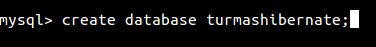
\includegraphics[scale=0.60]{CriandoBancoDeDados.png}
    \caption{Criando um banco de dados}
    \label{imagemCriandoBancodeDados}
\end{figure}

Crie um projeto WEB novo no Netbeans clicando em Arquivo $\rightarrow$ Novo Projeto $\rightarrow$ Java Web $\rightarrow$ Aplicação Web

\begin{figure}[H]
    \centering
    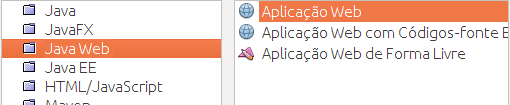
\includegraphics[scale=0.60]{NovoProjetoWeb.png}
    \caption{Criando um projeto novo}
    \label{imagemNovoProjetoWeb}
\end{figure}

Dê um nome para o projeto, selecione o Servidor de Aplicações Jboss e a última versão do Java instalada. Durante o desenvolvimento deste tutorial foi usado o Java EE 6.

\begin{figure}[H]
    \centering
    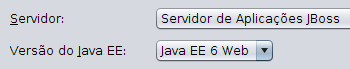
\includegraphics[scale=0.60]{jboss.png}
    \caption{Selecionando o servidor e a versão do Java}
    \label{imagemServidorVersaoJava}
\end{figure}

Na sessão seguinte selecione o \textit{framework} \textbf{JavaServerFace} e o componente \textbf{PrimeFaces}.

\begin{figure}[H]
    \centering
    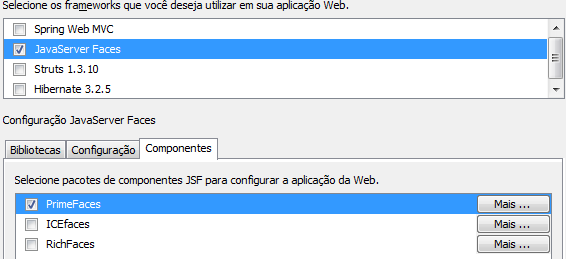
\includegraphics[scale=0.80]{SelectJavaServerFace.png}
    \caption{Selecionando o Framework}
    \label{imagemSelecionandoJavaServerFace}
\end{figure}

%Biblioteca não necessária no Tutorial 2!!!

%\textbf{Obs:} O Primeface necessita de uma biblioteca chamada commons-fileupload-1.3.jar para funcionar adequadamente. Essa biblioteca pode ser baixada diretamente do site da Apache:
%\url{http://commons.apache.org/proper/commons-fileupload}{Baixe aqui!}
%\textit{http://commons.apache.org/proper/commons-fileupload}\\
%Após fazer o download da biblioteca é necessário adicioná-la em seu projeto no Netbeans. Para isso prossiga até a aba Biblioteca $\rightarrow$ clique com o botão direito $\rightarrow$ e vá em adicionar JAR/Pasta procure o arquivo baixado e selecione-o.\\

%begin{figure}[H]
%    \centering
%    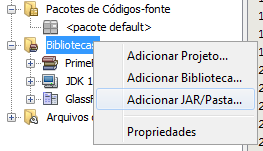
\includegraphics[scale=0.70]{adicionarJar}
%    \caption{Adicionando a biblioteca commons-fileupload}
%    \label{imagemAdicionarJar}
%\end{figure}


Em seguida selecione o \textbf{Hibernate}, mas não finalize ainda, é necessário configurar a conexão com o banco de dados. Essa etapa poderia ser feita posteriormente, mas é preferível já realizá-la nesse momento.\\

%Acrescentada explicação de como conectar o banco de dados usando o assistente de confiração do hibernate
Configurar Hibernate
\begin{enumerate}
\item{Conexão ao banco de dados}\\ %Editado!!!
Em Pacotes de Código-fonte selecione: Novo $\rightarrow$ Assistente de Configuração do Hibernate, deixe o nome do arquivo como hibernate.cfg e clique em next, selecione: Nova Conexão de Banco de Dados
\item{Driver}\\
Mysql (Conector/J driver)
\item{Assistente para nova Conexão}\\
Informe o nome do banco de dados, no caso turmashibernate, o nome do usuário e senha para esse banco. É possível verificar se as informações foram inseridas corretamente e se a conexão vai funcionar, clicando em "Testar Conexão".
\begin{figure}[H]
    \centering
    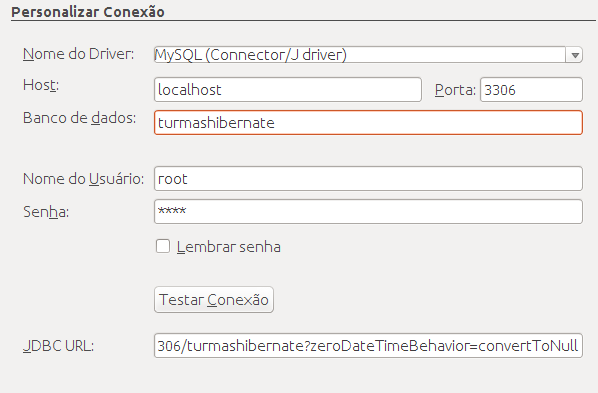
\includegraphics[scale=0.50]{ConfiguracaoConexao.png}
    \caption{Configuração da Conexão com o banco de dados}
    \label{imagemConfiguracaoConexao}
\end{figure}
\end{enumerate}

Após terminada a conexão com o banco de dados vá até a pasta Biblioteca e procure as bibliotecas PrimesFaces 5.0 e Hibernate 4.3.x e as exclua. Após isso adicione as seguintes bibliotecas:

\begin{figure}[H]
    \centering
    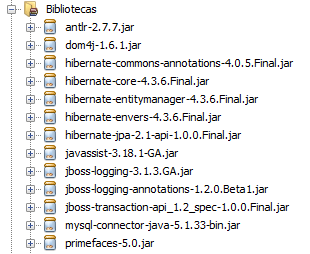
\includegraphics{bibliotecas.PNG}
    \caption{Bibliotecas}
    \label{imagembibliotecas}
\end{figure}

Essas bibliotecas podem ser baixadas do repositório desse tutorial no GitHub através dessa \href{https://github.com/julianacalio/Tutorial2/blob/master/Bibliotecas.zip}{\textbf{página}}. 

\textbf{Obs.: }Foram usadas as versões das bibliotecas mais atuais até o momento do desenvolvimento do código do projeto. Porém, novas versões podem ser lançadas e utilizadas posteriormente.

    
Agora já podemos finalizar as configurações iniciais.

Na pasta \textit{pacote default} o Netbeans criou um arquivo chamado hibernate.xfg.xml o qual contém a configuração do banco de dados.
Esse arquivo contém a configuração do banco de dados feita na etapa inicial da criação do projeto.



%codigo hibernate.cfg.xml
\lstset{language=HTML}
\begin{lstlisting}
<?xml version="1.0" encoding="UTF-8"?>
<!DOCTYPE hibernate-configuration PUBLIC "-//Hibernate/Hibernate Configuration DTD 3.0//EN" "http://hibernate.sourceforge.net/hibernate-configuration-3.0.dtd">
<hibernate-configuration>
  <session-factory>
    <property name="hibernate.dialect">org.hibernate.dialect.MySQLDialect</property>
    <property name="hibernate.connection.driver_class">com.mysql.jdbc.Driver</property>
    <property name="hibernate.connection.url">jdbc:mysql://localhost:3306/turmas29?zeroDateTimeBehavior=convertToNull</property>
    <property name="hibernate.connection.username">root</property>
    <property name="hibernate.connection.password">root</property>
  </session-factory>
</hibernate-configuration>
\end{lstlisting}

\newpage
\section{Estrutura das classes}

O projeto seguirá a mesma ideia do projeto desenvolvido no primeiro tutorial. Teremos um Modelo MVC e faremos uso do padrão de projeto Facade.

\subsection{Modelo}
Vamos criar inicialmente um pacote chamado modelo, no qual conterá nossas classes que cuidarão das regras de negócio do sistema.\\
Crie três classes chamadas Docente \ref{subsectionDocente}, Disciplina \ref{subsectionDisciplina} e uma última chamada Turma \ref{subsectionTurma}. Abaixo podemos ver o diagrama de classes que representa essa implementação.\\

\begin{figure}[H]
    \centering
    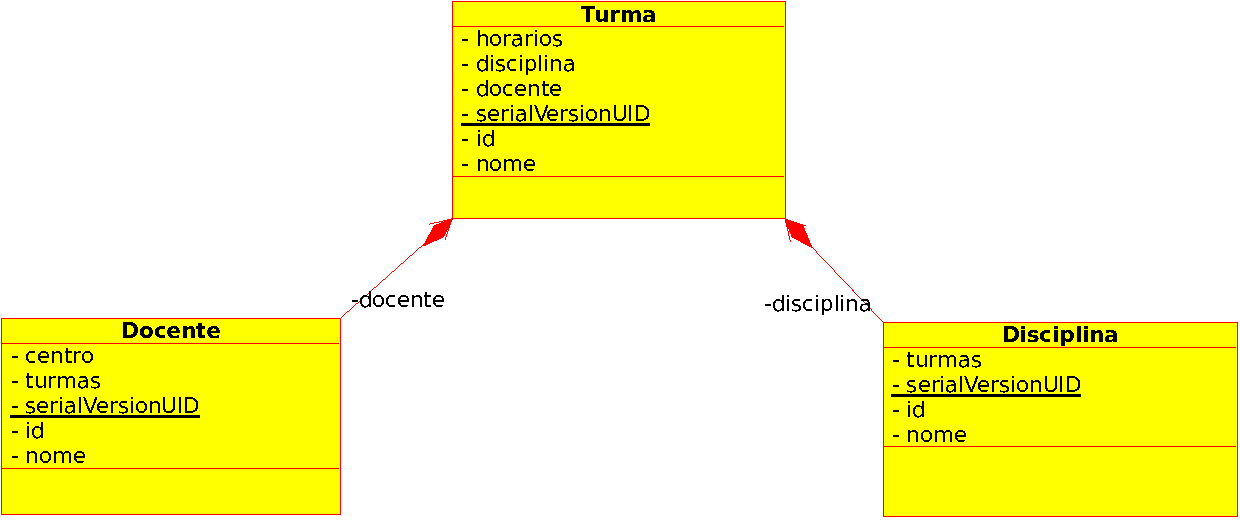
\includegraphics[scale=0.50]{DiagramaClasses.pdf}
    \caption{Diagrama de classes}
    \label{imagemDiagramaClasses}
\end{figure}

 A primeira coisa a ser observada neste exemplo de programa são as \textit{anotações do hibernate} que permitem fazer o mapeamento da classe para uma tabela do banco de dados. As anotações padrões do EJB estão contidas em um pacote chamado javax.persistence.\\

\textit{\textbf{@Entity Annotation:}}

A primeira anotação é a \textit{@Entity}. Ela associa o nome da Classe com uma tabela no banco de dados. Logo em seguida usamos a anotação @Entity para as classes Docente, Disciplina e Turma, a qual demarca estas classes como \textit{beans} de entidade, logo não deve haver um construtor visível sem argumentos ou no mínimo com escopo \textit{protected}. \\
%The EJB 3 standard annotations are contained in the javax.persistence package, so we import this package as the first step. Second we used the @Entity annotation to the Employee class which marks this class as an entity bean, so it must have a no-argument constructor that is visible with at least protected scope.\\

\textit{\textbf{@Id e @GeneratedValue Annotations:}}

%Each entity bean will have a primary key, which you annotate on the class with the @Id annotation. The primary key can be a single field or a combination of multiple fields depending on your table structure.
Cada entidade terá uma chave primária, que receberá a anotação @Id. A chave primária pode ser um campo único ou uma combinação de múltiplos campos dependendo da estrutura da tabela.


%By default, the @Id annotation will automatically determine the most appropriate primary key generation strategy to be used but you can override this by applying the @GeneratedValue annotation which takes two parameters strategy and generator which I'm not going to discuss here, so let us use only default the default key generation strategy. Letting Hibernate determine which generator type to use makes your code portable between different databases.\\

Por padrão, a anotação @Id irá automaticamente determinar a estratégia de geração de chave primária mais apropriada para ser usada, mas é possível sobreescrevê-la aplicando a anotação @GeneratedValue, que recebe dois parâmetros: \textit{strategy} e \textit{generator}.


As anotações @Id e @GeneratedValue fazem o mapeamento de identificação do banco de dados. O fornecedor de persistência do JPA detecta que a anotação @Id está em um campo e assume que ele deve acessar as propriedades de um objeto diretamente pelos campos em tempos de execução.\\

\textit{\textbf{@OneToMany Annotation:}}\\
A anotação \textit{@OneToMany} faz o mapeamento das turmas no docente.\\

É importante observar que as classes devem implementar a interface Serializable.
Agora precisamos identificar o mapeamento das classes no arquivo Hibernate.cfg.xml. Abra-o e acrescente as seguintes linhas abaixo da ultima "property":

\begin{lstlisting}
 		<mapping class="modelo.Docente"/>
        <mapping class="modelo.Disciplina"/>
        <mapping class="modelo.Turma"/>
\end{lstlisting}

Para completar a configuração deste arquivo é possível acrescentar alguns parâmetros, não obrigatórios, porém extremamente úteis, como por exemplo o monitoramento das instruções SQL executadas pelo Hibernate. Assim podemos ver como é resolvido o problema do $n+1$ selects. Para adicionar essa funcionalidade acrescente estes parâmetros no arquivo:
\begin{lstlisting}
		 <property name="hibernate.show_sql">true</property>
		 <property name="hibernate.format_sql">true</property>
		 <property name="hibernate.use_sql_comments">true</property>
		 <property name="hibernate.hbm2ddl.auto">update</property>
\end{lstlisting}


Outra opção é ir na aba \textit{Design} do arquivo Hibernate.cfg.xml e em Propriedades Opcionais $\rightarrow$ Propriedades de Configuração $\rightarrow$ Adicionar e adicionar as três primeiras propriedades mostradas anteriormente. 

\begin{figure} [!h]
\centering 
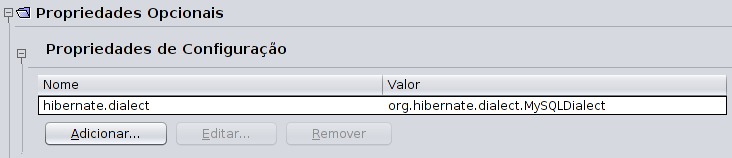
\includegraphics[width=0.7\linewidth]{2.png}
\caption{Propriedades de Configuração do Hibernate}
\label{fig:2}
\end{figure}

Para adicionar a última propriedade ("hibernate.hbm2ddl.auto"), vá em Propriedades Opcionais $\rightarrow$ Propriedades Diversas $\rightarrow$ Adicionar, como mostrado na Figura \ref{fig:3}.

\begin{figure} [h]
\centering
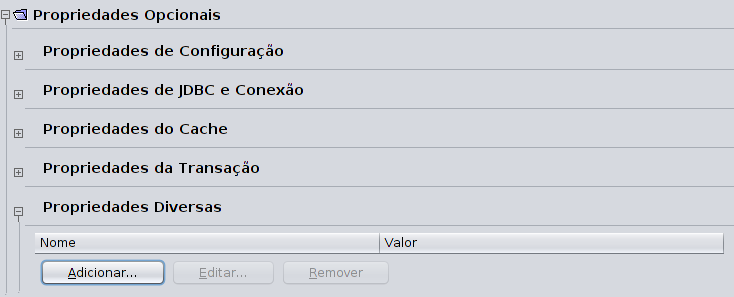
\includegraphics[width=0.7\linewidth]{3.png}
\caption{Propriedades diversas do Hibernate}
\label{fig:3}
\end{figure}


%Este arquivo de configuração tem uma segunda importância na automatização do processo de desenvolvimento. Baseado nas configurações do banco de dados desse arquivo, é possível usar uma ferramenta do hibernate para gerar o banco de dados a partir das classes mapeadas pelas anotações dele.\\
%Para fazer isso vamos criar inicialmente um pacote chamado Util. Dentro dele crie uma classe chamada GeraBanco. Coloque o código YYYYY e execute o programa.\\
%Depois disso podemos verificar como ficou o banco de dados. Abra o terminal de comando e digite o comando: \textit{Show tables}.
%Deverá ser mostrado todas tabelas Docente, Disciplina e Turma.
%
%\begin{figure}[H]
%    \centering
%    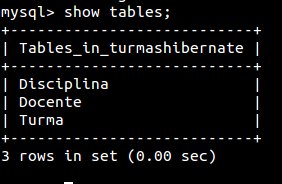
\includegraphics[scale=0.50]{Imagens/ShowTables.png}
%    \caption{Mostrando as tabelas criadas no banco de dados}
%    \label{imagemShowTables}
%\end{figure}

\subsection{Controller}
No pacote \textit{controller}, irão residir as classes que farão o controle das páginas de acesso ao usuário. Primeiramente crie uma classe chamada JsfUtil.java \ref{subsectionJsfUtil}. Essa classe cuidará de detalhes específicos das páginas como manipulação de mensagens de erros e a recuperação de itens na página.Essa classe servirá como base para todas as outras que manipularão as páginas JSF. 

Vamos começar criando a classe DocenteController \ref{subsectionDocenteController}.
Algumas observações devem ser feitas sobre essas classes. Perceba que algumas anotações apareceram agora, como, por exemplo, as duas anotações:
\lstset{language=JAVA}
\begin{lstlisting}
@Named(value = "docenteController")
@SessionScoped
public class DocenteController implements Serializable {

    public DocenteController() {
        docente = new Docente();
    }

    private Docente docente;

    @EJB
    private DocenteFacade docenteFacade;
    private static DocenteDataModel docenteDataModel;
\end{lstlisting}

A primeira mapeia um objeto da Classe DocenteController, que poderá ser usado nas páginas  \textit{xhtml}. A segunda especifica que um bean é escopo de sessão. A terceira marcação, \textbf{@EJB}, especifica o objeto docenteController que será injetado no código, e poderá ser usada nas páginas JSF sem precisar declarar o objeto.\\

Crie agora as classes DisciplinaController \ref{subsectionDisciplinaController} e TurmaController \ref{subsectionTurmaController}. Essas três classes não possuem nenhum algoritmo especial, somente métodos para fazer a interação com as páginas e com a camada \textit{facade}, que fará acesso ao banco de dados.


\subsection{Facade}
A camada \textit{facade} fará toda a parte de comunicação com o banco de dados. Como as três classes que iremos trabalhar irão interagir com o banco, iremos criar uma classe abstrata, \textit{AbstractFacade}, \ref{subsectionAbstractFacade} que irá generalizar as funcionalidades de inserção, remoção e atualização do banco de dados. Essa classe contém as funcionalidades básicas de um sistema CRUD em uma banco de dados.


 Crie agora a classe DocenteFacade \ref{subsectionDocenteFacade}, que herdará da classe \textit{AbstractFacade}. Nesta classe é usada a marcação @Stateless que indica que o estado da sessão do \textit{session bean} não devera ser mantido. Nela também é implementado o método \textit{getSectionFactory}, método abstrato declarado pela classe \textit{AbstractFacade}. Este método faz uso da função \textit{HibernateUtil.getSessionFactory()} que retorna um objeto sectionFactory. Em seguida crie as classes DisciplinaFacade \ref{subsectionDisciplinaFacade} e TurmaFacade \ref{subsectionTurmaFacade}, seguindo os mesmos passos utilizados para a criação da classe DocenteFacade.
 
 Implemente a classe HibernateUtil \ref{subsectionHibernateUtil}, para poder prosseguir no tutorial.
 Em seguida crie a Classe DocenteFacade \ref{subsectionDocenteFacade} DisciplinaFacade \ref{subsectionDisciplinaFacade} e TurmaFacade \ref{subsectionTurmaFacade}.
 
\subsection{Util}
Também será necessário criar um pacote chamado \textit{\textbf{util}}. Ele será criado do mesmo modo que os outros pacotes. Esse pacote possui os DataModels das entidades. O DataModel armazena uma coleção de objetos da entidade que irão popular o componente DataTable do Primefaces das páginas \textit{web}.

Dentro do pacote iremos criar uma classe chamada DocenteDataModel \ref{subsectionDocenteDataModel}. Essa classe irá interagir com a classe DocenteController.

Após isso também é necessário criar as classes DisciplinaDataModel \ref{subsectionDisciplinaDataModel} e TurmaDataModel \ref{subsectionTurmaDataModel}.

\newpage
\section{Páginas Web}

Agora podemos começar a modelar as páginas \textit{web}. Embora tenhamos feito muito código antes de chegar nesta parte, todo este trabalho começará a fazer sentido agora.
Fazer páginas \textit{web} não requer muito trabalho, mas pode causar uma certa insegurança inicial para quem nunca trabalhou com este tipo de tecnologia. Iremos fazer todo o desenho via código, sem usar ferramentas "drag and drop", assim ficará claro o que cada linha código significa. \\


\hrule
\hrulefill\\
\textit{Obs.:É fortemente recomendado que qualquer código deste tutorial seja digitado pelo programador e não simplesmente copiado e colado. Ao fazer a digitação as funcionalidades de autocomplete da IDE irão poder te guiar se está saindo tudo certo ou se tem algo errado.}\\
\hrule
\hrulefill\\


\subsection{Criando o índex - A primeira página}

Como já deve ter sido notado, o \textbf{índex} é criado automaticamente pelo Netbeans. Vamos fazer algumas alterações nele e deixá-lo da seguinte forma:

\lstset{language=HTML}
\begin{lstlisting}
<?xml version='1.0' encoding='UTF-8' ?>
<!DOCTYPE html PUBLIC "-//W3C//DTD XHTML 1.0 Transitional//EN" "http://www.w3.org/TR/xhtml1/DTD/xhtml1-transitional.dtd">
<html xmlns="http://www.w3.org/1999/xhtml"
      xmlns:h="http://java.sun.com/jsf/html"
      xmlns:f="http://java.sun.com/jsf/core"
      xmlns:p="http://primefaces.org/ui">
    <h:head>
        <title>Facelet Title</title>
    </h:head>
    <h:body>
        <f:view>
            <h:form style="background-color: transparent">
                <p:panel id="conpnl" header="Index"  style="width:280px;height:300px; border-color: transparent; position: relative; left: 530px; text-align: center; background-color: transparent">
                    <br/>
                    <p:panelMenu style="width:250px; height: 300px; text-align: justify; position: relative; ">
                        <p:submenu label="Docentes">
                            <p:menuitem value="Listar todos os docentes" action="/view/docente/List" icon="ui-icon-document" />
                            <p:menuitem value="Cadastrar um docente" action="#{docenteController.prepareCreate()}" icon="ui-icon-disk"/>
                        </p:submenu>
                        <p:submenu  label="Disciplinas">
                            <p:menuitem value="Listar todas as disciplinas" action="/view/disciplina/List" icon="ui-icon-document" />
                            <p:menuitem value="Cadastrar uma disciplina" action="#{disciplinaController.prepareCreate()}" icon="ui-icon-disk"/>
                        </p:submenu>
                        <p:submenu label="Turmas">
                            <p:menuitem value="Listar todas as turmas" action="/view/turma/List" icon="ui-icon-document" />
                            <p:menuitem value="Cadastrar uma turma" action="#{turmaController.prepareCreate()}" icon="ui-icon-disk"/>
                        </p:submenu>
                    </p:panelMenu>
                </p:panel>
            </h:form>
        </f:view>
    </h:body>
</html>
\end{lstlisting}

Esta é uma página bem simples que gera três links que direcionarão para outras três páginas. Vamos criar um estrutura de pastas para colocar as demais páginas que farão parte dessa aplicação.\\
Crie uma pasta chamada \textbf{view}. Dentro dela coloque outras 3 pastas, docente, disciplina e turma. 

\begin{figure}[!htb]
    \centering
    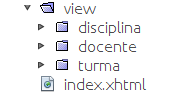
\includegraphics[scale=0.60]{pastas.png}
    \caption{Estrutura das pastas}
    \label{imagemEstruturaPastasView}
\end{figure}



\subsection{Criando Todas as Páginas}
Nesse ponto, os links ainda não responderão, pois as páginas para as quais eles direcionam ainda não estão criadas. Vamos criá-las agora. Na pasta \textbf{docente} crie os seguintes arquivos: Create.xhtml \ref{subsubsectionDocenteCreate}, Edit.xhtml \ref{subsubsectionDocenteEdit}, List.xhtml \ref{subsubsectionDocenteList}.\\
O código destas páginas possui as particularidades da linguagem \textit{html} e está fora do escopo deste segundo tutorial explicá-las detalhadamente. Entretanto, é preciso chamar a atenção da forma que os métodos da classe DocenteController são chamados:
\lstset{language=HTML}
\begin{lstlisting}
#{docenteController.docente.nome}
\end{lstlisting}
No exemplo acima é acessado o objeto docenteController que acessa o método getDocente e depois getNome.\\


Faça a mesma coisa nas pastas \textbf{disciplina} e \textbf{turma}, criando os arquivos Create \ref{subsubsectionDisciplinaCreate}, Edit \ref{subsubsectionDisciplinaEdit}, List \ref{subsubsectionDisciplinaList} para Disciplina e novamente Create \ref{subsubsectionTurmaCreate}, Edit \ref{subsubsectionTurmaEdit}, List \ref{subsubsectionTurmaList} para Turma.

\newpage
\section{Colocando a Aplicação para Funcionar}
Assim como no tutorial anterior este programa tem funcionalidades bem simples que podem ser testadas criando ou excluindo Docentes, Disciplinas ou Turmas. Ao rodar a aplicação, deve aparecer uma página de índice.

\begin{figure}[H]
    \centering
    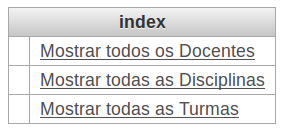
\includegraphics[scale=0.50]{index.png}
    \caption{Pagina inicial}
    \label{imagemindex}
\end{figure}

Para testar o código vamos criar um docente, uma disciplina e uma turma. Para criar o docente vá em Mostrar todos os docentes $\rightarrow$ Criar um Docente. Insira o nome do docente e clique em Cadastrar Docente.

\begin{figure}[H]
    \centering
    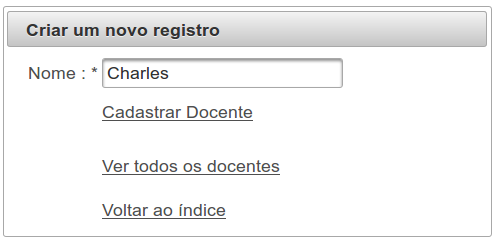
\includegraphics[scale=0.45]{criarDocente.png}
    \caption{Cadastro de um docente}
    \label{criarDocente}
\end{figure}

Se o cadastro foi realizado com sucesso, aparecerá a seguinte mensagem:
\begin{figure}[H]
    \centering
    
\includegraphics[scale=0.50]{mensagemSucesso.png}
    \caption{Cadastramento realizado com sucesso}
    \label{mensagemSucesso}
\end{figure}

Para visualizar o docente recém criado, clique em Ver todos os docentes.\\

\begin{figure}[H]
    \centering
    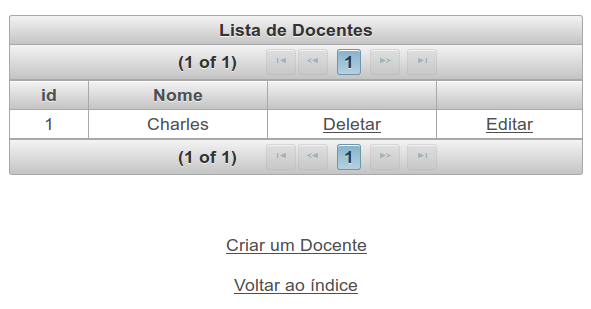
\includegraphics[scale=0.45]{listDocente.png}
    \caption{Visualização de todos os docentes}
    \label{listDocente}
\end{figure}

Para criar uma disciplina vá em Mostrar todas as disciplinas $\rightarrow$ Criar uma Disciplina. Insira o nome da disciplina e clique em Cadastrar Disciplina.

\begin{figure}[H]
    \centering
    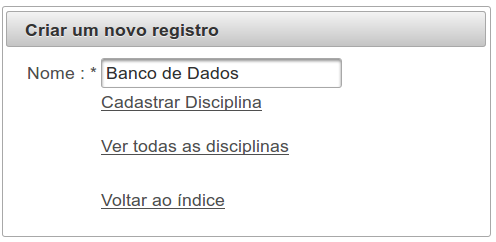
\includegraphics[scale=0.45]{criarDisciplina.png}
    \caption{Cadastro de uma disciplina}
    \label{criarDisciplina}
\end{figure}

Se o cadastro foi realizado com sucesso, aparecerá a uma mensagem semelhante à exibida no cadastro do Docente. Para visualizar a disciplina criada, clique em Ver todas as disciplinas.

\begin{figure}[H]
    \centering
    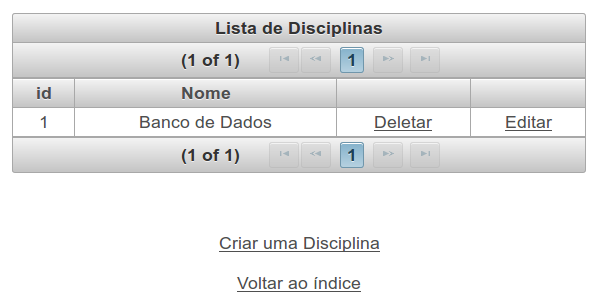
\includegraphics[scale=0.45]{listDisciplina.png}
    \caption{Visualização de todas as disciplinas}
    \label{listDisciplina}
\end{figure}
 
Finalmente, para criar uma turma vá em Mostrar todas as turmas $\rightarrow$ Criar uma Turma. Escolha um docente e uma disciplina para essa turma nas \textit{combo boxes} e clique em Cadastrar Turma.

\begin{figure}[H]
    \centering
    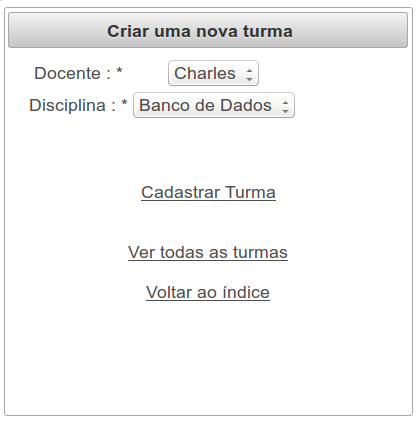
\includegraphics[scale=0.45]{criarTurma.png}
    \caption{Cadastro de uma turma}
    \label{criarTurma}
\end{figure}

Se o cadastro foi realizado com sucesso, aparecerá a uma mensagem semelhante à exibida nos cadastros do Docente e da Disciplina. Para visualizar a turma criada, clique em Ver todas as turmas.

\begin{figure}[H]
    \centering
    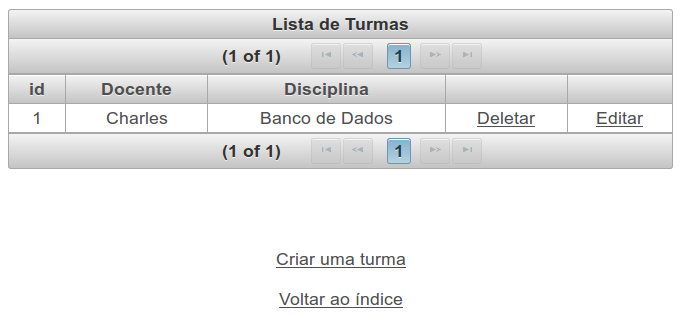
\includegraphics[scale=0.45]{listTurma.png}
    \caption{Visualização de todas as turmas}
    \label{listTurma}
\end{figure}

Nesse ponto, podemos chamar a atenção para o problema do $n+1$ \textit{selects} que foi abordado no começo deste tutorial. É fácil verificar como ele foi resolvido pelo \textit{Hibernate}, através do \textbf{carregamento ansioso} das associações. Abra a página para Listar todas as turmas e veja saída do Hibernate, mostrando a instrução SQL gerada:
\lstset{language=SQL}
\begin{lstlisting}
 /* criteria query */ select
          this_.ID as ID1_2_2_,
          this_.disciplina_ID as discipli2_2_2_,
          this_.docente_ID as docente_3_2_2_,
          disciplina2_.ID as ID1_0_0_,
          disciplina2_.nome as nome2_0_0_,
          docente3_.ID as ID1_1_1_,
          docente3_.nome as nome2_1_1_ 
      from
          Turma this_ 
      left outer join
          Disciplina disciplina2_ 
              on this_.disciplina_ID=disciplina2_.ID 
      left outer join
          Docente docente3_ 
              on this_.docente_ID=docente3_.ID
\end{lstlisting}

O carregamento ansioso é habilitado através do parâmetro fetch = FetchType.EAGER da notação de associação @OneToMany presente nas classes Docente \ref{subsectionDocente} e Disciplina \ref{subsectionDisciplina}, para fazer a associação das mesmas com a classe Turma. Dessa forma, ao invés de fazer vários selects individuais para recuperar o docente e a disciplina de cada turma, o Hibernate faz um \textit{\textbf{left outer join}} para buscar todos os dados com um única instrução.\\


Para ilustrar as funções Edit e Delete, vamos criar mais um docente.

\begin{figure}[H]
    \centering
    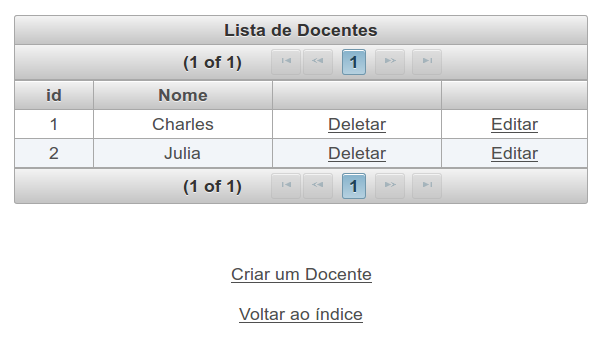
\includegraphics[scale=0.45]{criarDocente2.png}
    \caption{Visualização de todos os docentes}
    \label{criarDocente2}
\end{figure}

Ao clicar em Editar, é aberta uma nova página, onde é possível editar as informações do docente escolhido. Vamos trocar o nome para Juliana e clicar em Editar Docente.
\begin{figure}[H]
    \centering
    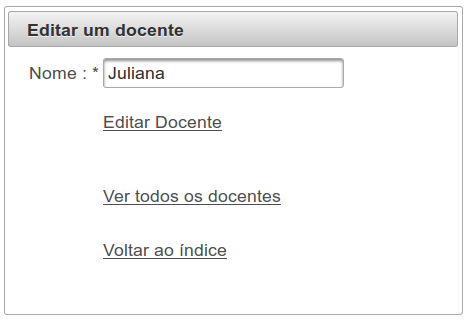
\includegraphics[scale=0.45]{editarDocente2.png}
    \caption{Editar Docente}
    \label{editarDocente2}
\end{figure}

Após a confirmação de que o docente foi editado com sucesso, podemos clicar em Ver todos os docentes para verificar se ele realmente foi modificado.

\begin{figure}[H]
    \centering
    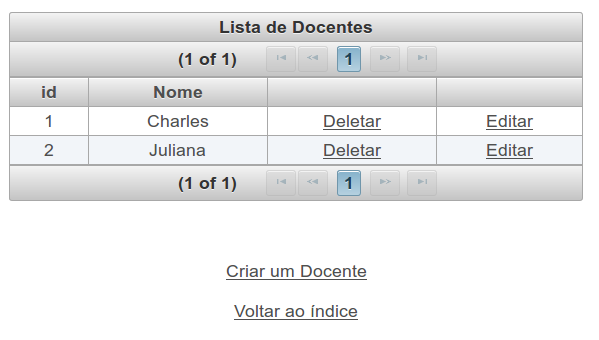
\includegraphics[scale=0.45]{visualizarDocente3.png}
    \caption{Visualização de todos os docentes}
    \label{visualizarDocente3}
\end{figure}

Para apagar o docente, basta clicar em deletar.

\begin{figure}[H]
    \centering
    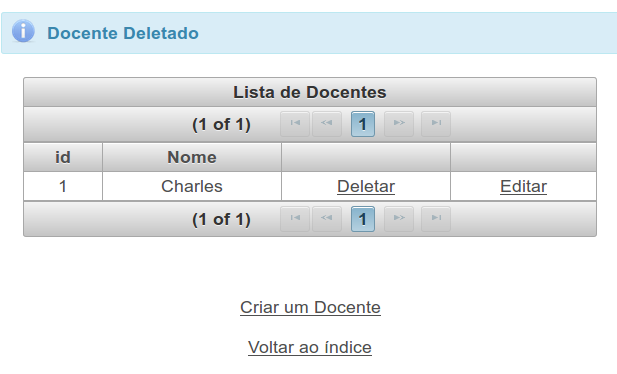
\includegraphics[scale=0.45]{delete.png}
    \caption{Visualização de todos os docentes após o delete}
    \label{delete}
\end{figure}

\newpage
\section{Apêndice Códigos Fonte}

Esse Apêndice tem o código de todas as classes java e páginas web desenvolvidos no tutorial.
\label{sectionCodigosFonte}

\subsection{Docente}
\label{subsectionDocente}
\lstset{language=JAVA}
\begin{lstlisting}
package model;

import java.io.Serializable;
import java.util.List;
import javax.persistence.CascadeType;
import javax.persistence.Entity;
import javax.persistence.FetchType;
import javax.persistence.GeneratedValue;
import javax.persistence.GenerationType;
import javax.persistence.Id;
import javax.persistence.OneToMany;

@Entity
public class Docente implements Serializable {

    private static final long SerialVersionUID = 1L;

    public Docente() {

    }

    @Id
    @GeneratedValue(strategy = GenerationType.AUTO)
    private Long ID;

    public Long getID() {
        return ID;
    }

    public void setID(Long ID) {
        this.ID = ID;
    }

    private String nome;

    public String getNome() {
        return nome;
    }

    public void setNome(String nome) {
        this.nome = nome;
    }

    @OneToMany(cascade = CascadeType.ALL, mappedBy = "docente", fetch = FetchType.EAGER)
    private List<Turma> turmas;

    public List<Turma> getTurmas() {
        return turmas;
    }

    public void setTurmas(List<Turma> turmas) {
        this.turmas = turmas;
    }

    @Override
    public int hashCode() {
        int hash = 0;
        hash += (ID != null ? ID.hashCode() : 0);
        return hash;

    }

    @Override
    public boolean equals(Object object) {

        if (!(object instanceof Docente)) {
            return false;
        }

        Docente other = (Docente) object;
        if ((this.ID == null && other.ID != null) || (this.ID != null && !(this.ID.equals(other.ID)))) {
            return false;
        }

        return true;

    }

    @Override
    public String toString() {
        return this.nome;
    }

}
\end{lstlisting}

\subsection{Disciplina}
\label{subsectionDisciplina}
\begin{lstlisting}
package model;

import java.io.Serializable;
import java.util.List;
import javax.persistence.CascadeType;
import javax.persistence.Entity;
import javax.persistence.FetchType;
import javax.persistence.GeneratedValue;
import javax.persistence.GenerationType;
import javax.persistence.Id;
import javax.persistence.OneToMany;

@Entity
public class Disciplina implements Serializable {

    private static final long SerialVersionUID = 1L;

    public Disciplina() {

    }

    @Id
    @GeneratedValue(strategy = GenerationType.AUTO)
    private Long ID;

    public Long getID() {
        return ID;
    }

    public void setID(Long ID) {
        this.ID = ID;
    }

    private String nome;

    public String getNome() {
        return nome;
    }

    public void setNome(String nome) {
        this.nome = nome;
    }

    @OneToMany(cascade = CascadeType.ALL, mappedBy = "disciplina", fetch = FetchType.EAGER)
    private List<Turma> turmas;

    public List<Turma> getTurmas() {
        return turmas;
    }

    public void setTurmas(List<Turma> turmas) {
        this.turmas = turmas;
    }

    @Override
    public int hashCode() {
        int hash = 0;
        hash += (ID != null ? ID.hashCode() : 0);
        return hash;

    }

    @Override
    public boolean equals(Object object) {

        if (!(object instanceof Disciplina)) {
            return false;
        }

        Disciplina other = (Disciplina) object;
        if ((this.ID == null && other.ID != null) || (this.ID != null && !(this.ID.equals(other.ID)))) {
            return false;
        }

        return true;

    }

    @Override
    public String toString() {
        return this.nome;
    }

}
\end{lstlisting}

\subsection{Turma}
\label{subsectionTurma}
\begin{lstlisting}
package model;

import java.io.Serializable;
import javax.persistence.Entity;
import javax.persistence.GeneratedValue;
import javax.persistence.GenerationType;
import javax.persistence.Id;
import javax.persistence.ManyToOne;

@Entity
public class Turma implements Serializable {

    public Turma() {

    }

    private static final long SerialVersionUID = 1L;

    @Id
    @GeneratedValue(strategy = GenerationType.AUTO)
    private Long ID;

    public Long getID() {
        return ID;
    }

    public void setID(Long ID) {
        this.ID = ID;
    }

    @ManyToOne
    private Disciplina disciplina;

    public Disciplina getDisciplina() {
        return disciplina;
    }

    public void setDisciplina(Disciplina disciplina) {
        this.disciplina = disciplina;
    }

    @ManyToOne
    private Docente docente;

    public Docente getDocente() {
        return docente;
    }

    public void setDocente(Docente docente) {
        this.docente = docente;
    }

    @Override
    public int hashCode() {
        int hash = 0;
        hash += (ID != null ? ID.hashCode() : 0);
        return hash;

    }

    @Override
    public boolean equals(Object object) {

        if (!(object instanceof Turma)) {
            return false;
        }

        Turma other = (Turma) object;
        if ((this.ID == null && other.ID != null) || (this.ID != null && !(this.ID.equals(other.ID)))) {
            return false;
        }

        return true;

    }

    @Override
    public String toString() {
        return ("model.Turma[ id = " + this.ID + " ]");
    }

}
\end{lstlisting}

\subsection{HibernateUtil}
\label{subsectionHibernateUtil}
\begin{lstlisting}

package controller;

import org.hibernate.Session;
import org.hibernate.SessionFactory;
import org.hibernate.boot.registry.StandardServiceRegistryBuilder;
import org.hibernate.cfg.Configuration;


public class HibernateUtil {

    private static final SessionFactory sessionFactory;

    static {
        try {
            
            
            Configuration configuration = new Configuration();
            configuration.configure("hibernate.cfg.xml");
            StandardServiceRegistryBuilder ssrb = new StandardServiceRegistryBuilder().applySettings(configuration.getProperties());
             sessionFactory = configuration.buildSessionFactory(ssrb.build());
            Session session = sessionFactory.openSession();

        } catch (Throwable ex) {
            // Log the exception. 
            System.err.println("Initial SessionFactory creation failed." + ex);
            throw new ExceptionInInitializerError(ex);
        }
    }

    public static SessionFactory getSessionFactory() {
        return sessionFactory;
    }
}


\end{lstlisting}

\subsection{AbstractFacade}
\label{subsectionAbstractFacade}
\begin{lstlisting}

package facade;

import java.util.List;
import org.hibernate.Criteria;
import org.hibernate.Session;
import org.hibernate.SessionFactory;
import org.hibernate.Transaction;
import org.hibernate.criterion.Projections;


public abstract class AbstractFacade<T> {

    private Class<T> entityClass;

    public AbstractFacade(Class<T> entityClass) {
        this.entityClass = entityClass;
    }

    protected abstract SessionFactory getSessionFactory();

    public void save(T entity) {
        Session session = getSessionFactory().openSession();
        Transaction transaction = session.beginTransaction();
        session.save(entity);
        transaction.commit();
        session.close();
    }

    public void edit(T entity) {
        Session session = getSessionFactory().openSession();
        Transaction transaction = session.beginTransaction();
        session.update(entity);
        transaction.commit();
        session.close();
    }

    public void remove(T entity) {
        Session session = getSessionFactory().openSession();
        Transaction transaction = session.beginTransaction();
        session.delete(entity);
        transaction.commit();
        session.close();
    }

    public T find(Long id) {
        Session session = getSessionFactory().openSession();
        T entity = (T) session.get(entityClass, id);
        session.close();
        return entity;
    }

    public List<T> findAll() {
        Session session = getSessionFactory().openSession();
        Criteria crit = session.createCriteria(entityClass);
        crit.setMaxResults(50);
        List results = crit.list();
        session.close();
        return results;
    }

    public List<T> findRange(int[] range) {
        Session session = getSessionFactory().openSession();
        Criteria crit = session.createCriteria(entityClass);
        crit.setMaxResults(range[1] - range[0]);
        crit.setFirstResult(range[0]);
        List results = crit.list();
        session.close();
        return results;
    }

    public int count() {
        Session session = getSessionFactory().openSession();
        Criteria crit = session.createCriteria(entityClass);
        int count = ((Number)crit.setProjection(Projections.rowCount()).uniqueResult()).intValue();
        session.close();
        return count;
    }
}

\end{lstlisting}

\subsection{DocenteFacade}
\label{subsectionDocenteFacade}
\begin{lstlisting}
package facade;

import controller.HibernateUtil;
import javax.ejb.Stateless;
import modelo.Docente;
import org.hibernate.SessionFactory;

@Stateless
public class DocenteFacade extends AbstractFacade<Docente> {

    @Override
    protected SessionFactory getSessionFactory() {
        return HibernateUtil.getSessionFactory();
    }

    public DocenteFacade() {
        super(Docente.class);
    }
}

\end{lstlisting}

\subsection{DisciplinaFacade}
\label{subsectionDisciplinaFacade}
\begin{lstlisting}
package facade;

import controller.HibernateUtil;
import javax.ejb.Stateless;
import modelo.Disciplina;
import org.hibernate.SessionFactory;

@Stateless
public class DisciplinaFacade extends AbstractFacade<Disciplina> {

    public DisciplinaFacade() {
        super(Disciplina.class);
    }

    @Override
    protected SessionFactory getSessionFactory() {
        return HibernateUtil.getSessionFactory();
    }
}

\end{lstlisting}

\subsection{TurmaFacade}
\label{subsectionTurmaFacade}
\begin{lstlisting}
package facade;

import controller.HibernateUtil;
import javax.ejb.Stateless;
import modelo.Turma;
import org.hibernate.SessionFactory;

@Stateless
public class TurmaFacade extends AbstractFacade<Turma> {

    public TurmaFacade() {
        super(Turma.class);
    }

    @Override
    protected SessionFactory getSessionFactory() {
        return HibernateUtil.getSessionFactory();
    }
}

\end{lstlisting}

\subsection{DocenteController}
\label{subsectionDocenteController}
\begin{lstlisting}
package controller;

import facade.DocenteFacade;
import java.io.Serializable;
import java.util.List;
import javax.ejb.EJB;
import javax.enterprise.context.SessionScoped;
import javax.faces.component.UIComponent;
import javax.faces.context.FacesContext;
import javax.faces.convert.Converter;
import javax.faces.convert.FacesConverter;
import javax.faces.model.SelectItem;
import javax.inject.Named;
import model.Docente;
import model.Turma;
import util.DocenteDataModel;

@Named(value = "docenteController")
@SessionScoped
public class DocenteController implements Serializable {

    public DocenteController() {
        docente = new Docente();
    }

    //Guarda o docente atual
    private Docente docente;

    @EJB
    private DocenteFacade docenteFacade;
    private static DocenteDataModel docenteDataModel;

    public void setDocente(Docente docente) {
        this.docente = docente;
    }

    private Docente getDocente(Long key) {
        return this.find(key);

    }

    public Docente getDocente() {
        if (docente == null) {
            docente = new Docente();
        }
        return docente;
    }

    public List<Turma> getTurmas() {
        return docente.getTurmas();
    }

    public SelectItem[] getItemsAvaiableSelectOne() {
        return JsfUtil.getSelectItems(docenteFacade.findAll(), true);
    }

    //Data Model*********************************************
    
    public DocenteDataModel getDocenteDataModel() {
        if (DocenteController.docenteDataModel == null) {
           
            List<Docente> docentes = this.findAll();
            DocenteController.docenteDataModel = new DocenteDataModel(docentes);
        }
        return DocenteController.docenteDataModel;
    }

    public static void setDocenteDataModel(DocenteDataModel docenteDataModel) {
        DocenteController.docenteDataModel = docenteDataModel;
    }

    public void recriarModelo() {
        DocenteController.docenteDataModel = null;
    }

    //"Prepares" das paginas*********************************
    
    public String prepareCreate() {
        docente = new Docente();
        return "Create";    
    }

    public String prepareEdit() {
        docente = (Docente) docenteDataModel.getRowData();
        return "Edit";
    }
    
    public String prepareList(){
        recriarModelo();
        return "List";
    }

    //CRUD***************************************************
    public String create() {

        try {
            docenteFacade.save(docente);
            JsfUtil.addSuccessMessage("Docente " + docente.getNome() + " criado com sucesso!");
            return prepareCreate();
        } catch (Exception e) {
            JsfUtil.addErrorMessage(e, "Ocorreu um erro de persistencia para salvar o docente " + docente.getNome());
            return null;
        }
    }

    public Docente find(Long id) {

        return docenteFacade.find(id);
    }

    private List<Docente> findAll() {
        return docenteFacade.findAll();

    }

    public void update() {
        try {
            docenteFacade.edit(docente);
            JsfUtil.addSuccessMessage("Docente Editado com sucesso!");
            docente = null;
        } catch (Exception e) {
            JsfUtil.addErrorMessage(e, "Ocorreu um erro de persistencia, nao foi possivel editar o docente: " + e.getMessage());

        }
    }

    public void delete() {
        docente = (Docente) docenteDataModel.getRowData();
        try {
            docenteFacade.remove(docente);
            docente = null;
            JsfUtil.addSuccessMessage("Docente Deletado");
        } catch (Exception e) {
            JsfUtil.addErrorMessage(e, "Ocorreu um erro de persistencia: " + e.getMessage() + " para deletar o docente " + docente.getNome());
        }

        recriarModelo();
    }

    //*******************************************************
    
    @FacesConverter(forClass = Docente.class)
    public static class DocenteControllerConverter implements Converter {

        @Override
        public Object getAsObject(FacesContext facesContext, UIComponent component, String value) {
            if (value == null || value.length() == 0) {
                return null;
            }
            DocenteController controller = (DocenteController) facesContext.getApplication().getELResolver().
                    getValue(facesContext.getELContext(), null, "docenteController");
            return controller.getDocente(getKey(value));
        }

        java.lang.Long getKey(String value) {
            java.lang.Long key;
            key = Long.valueOf(value);
            return key;
        }

        String getStringKey(java.lang.Long value) {
            StringBuilder sb = new StringBuilder();
            sb.append(value);
            return sb.toString();
        }

        @Override
        public String getAsString(FacesContext facesContext, UIComponent component, Object object) {
            if (object == null) {
                return null;
            }
            if (object instanceof Docente) {
                Docente d = (Docente) object;
                return getStringKey(d.getID());
            } else {
                throw new IllegalArgumentException("object " + object + " is of type " + object.getClass().getName() + "; expected type: " + Docente.class.getName());
            }
        }
    }

}
\end{lstlisting}

\subsection{DisciplinaController}
\label{subsectionDisciplinaController}
\begin{lstlisting}
package controller;

import facade.DisciplinaFacade;
import java.io.Serializable;
import java.util.List;
import javax.ejb.EJB;
import javax.enterprise.context.SessionScoped;
import javax.faces.component.UIComponent;
import javax.faces.context.FacesContext;
import javax.faces.convert.Converter;
import javax.faces.convert.FacesConverter;
import javax.faces.model.SelectItem;
import javax.inject.Named;
import model.Disciplina;
import util.DisciplinaDataModel;

@Named(value = "disciplinaController")
@SessionScoped
public class DisciplinaController implements Serializable {

    private Disciplina disciplina;

    @EJB
    DisciplinaFacade disciplinaFacade;
    private static DisciplinaDataModel disciplinaDataModel;

    public DisciplinaController() {
        this.disciplina = new Disciplina();
    }

    public Disciplina getDisciplina() {
        if (disciplina == null) {
            disciplina = new Disciplina();
        }
        return disciplina;
    }

    private Disciplina getDisciplina(Long key) {
        return this.find(key);
    }

    public SelectItem[] getItemsAvaiableSelectOne() {
        return JsfUtil.getSelectItems(disciplinaFacade.findAll(), true);
    }

    public void setDisciplina(Disciplina disciplina) {
        this.disciplina = disciplina;
    }

    //Data Model*********************************************
    
    public DisciplinaDataModel getDisciplinaDataModel() {
        if (disciplinaDataModel == null) {
            List<Disciplina> disciplinas = this.findAll();
            disciplinaDataModel = new DisciplinaDataModel(disciplinas);
        }
        return disciplinaDataModel;
    }

    public static void setDisciplinaDataModel(DisciplinaDataModel disciplinaDataModel) {
        DisciplinaController.disciplinaDataModel = disciplinaDataModel;
    }

    public void recriarModelo() {
        DisciplinaController.disciplinaDataModel = null;
    }

    //"Prepares" das paginas*********************************
    
    public String prepareCreate() {
        disciplina = new Disciplina();
            return "Create";
    }

    public String prepareEdit() {
        disciplina = (Disciplina) disciplinaDataModel.getRowData();
        return "Edit";
    }
    
    public String prepareList(){
        recriarModelo();
        return "List";
    }

    //CRUD***************************************************
   
    public String create() {

        try {
            disciplinaFacade.save(disciplina);
            JsfUtil.addSuccessMessage("Disciplina " + disciplina.getNome() + " criada com sucesso!");
            return prepareCreate();
        } catch (Exception e) {
            JsfUtil.addErrorMessage(e, "Ocorreu um erro de persistencia para salvar a disciplina " + disciplina.getNome());
            return null;

        }

    }

    public Disciplina find(Long id) {

        return disciplinaFacade.find(id);

    }

    public List<Disciplina> findAll() {
        return disciplinaFacade.findAll();
    }
    
    public void update() {
        try {
            disciplinaFacade.edit(disciplina);
            JsfUtil.addSuccessMessage("Disciplina editada com sucesso!");
            disciplina = null;

        } catch (Exception e) {
            JsfUtil.addErrorMessage(e, "Ocorreu um erro: " + e.getMessage() + " para editar a disciplina " + disciplina.getNome());
        }

    }

    public void delete() {
        disciplina = (Disciplina) disciplinaDataModel.getRowData();
        try {
            disciplinaFacade.remove(disciplina);
            disciplina = null;
            JsfUtil.addSuccessMessage("Disciplina Deletada");
        } catch (Exception e) {
            JsfUtil.addErrorMessage(e, "Ocorreu um erro de persistencia para deletar a disciplina " + disciplina.getNome());
        }
        recriarModelo();

    }

    //*******************************************************
    @FacesConverter(forClass = Disciplina.class)
    public static class DisciplinaControllerConverter implements Converter {

        @Override
        public Object getAsObject(FacesContext facesContext, UIComponent component, String value) {
            if (value == null || value.length() == 0) {
                return null;
            }
            DisciplinaController controller = (DisciplinaController) facesContext.getApplication().getELResolver().
                    getValue(facesContext.getELContext(), null, "disciplinaController");
            return controller.getDisciplina(getKey(value));
        }

        java.lang.Long getKey(String value) {
            java.lang.Long key;
            key = Long.valueOf(value);
            return key;
        }

        String getStringKey(java.lang.Long value) {
            StringBuilder sb = new StringBuilder();
            sb.append(value);
            return sb.toString();
        }

        @Override
        public String getAsString(FacesContext facesContext, UIComponent component, Object object) {
            if (object == null) {
                return null;
            }
            if (object instanceof Disciplina) {
                Disciplina d = (Disciplina) object;
                return getStringKey(d.getID());
            } else {
                throw new IllegalArgumentException("object " + object + " is of type " + object.getClass().getName() + "; expected type: " + Disciplina.class.getName());
            }
        }
    }

}
\end{lstlisting}

\subsection{TurmaController}
\label{subsectionTurmaController}
\begin{lstlisting}
package controller;

import facade.TurmaFacade;
import java.io.Serializable;
import java.util.List;
import javax.ejb.EJB;
import javax.enterprise.context.SessionScoped;
import javax.faces.component.UIComponent;
import javax.faces.context.FacesContext;
import javax.faces.convert.Converter;
import javax.faces.convert.FacesConverter;
import javax.inject.Named;
import model.Turma;
import util.TurmaDataModel;

@Named(value = "turmaController")
@SessionScoped
public class TurmaController implements Serializable {

    private Turma turma;

    @EJB
    private TurmaFacade turmaFacade;
    private TurmaDataModel turmaDataModel;

    public TurmaController() {
        turma = new Turma();

    }

    public Turma getTurma() {
        if (turma == null) {
            turma = new Turma();
        }
        return turma;
    }

    private Turma getTurma(Long key) {
        return this.find(key);

    }

    public void setTurma(Turma turma) {
        this.turma = turma;
    }

    //"Prepares" das paginas*********************************
    public String prepareCreate() {
        turma = new Turma();
        return "Create";

    }

    public String prepareEdit() {
        turma = (Turma) turmaDataModel.getRowData();
        return "Edit";
    }

    public String prepareList() {
        recriarModelo();
        return "List";
    }

    //DataModel**********************************************
    
    public TurmaDataModel getTurmaDataModel() {
        if (turmaDataModel == null) {
            List<Turma> turmas = this.findAll();
            turmaDataModel = new TurmaDataModel(turmas);
        }
        return turmaDataModel;
    }

    public void setTurmaDataModel(TurmaDataModel turmaDataModel) {
        this.turmaDataModel = turmaDataModel;
    }

    public void recriarModelo() {
        this.turmaDataModel = null;
    }

    //CRUD***************************************************
    
    public String create() {

        try {
            turmaFacade.save(turma);
            JsfUtil.addSuccessMessage("Turma " + turma.getID() + " criada com sucesso!");
            return prepareCreate();
        } catch (Exception e) {
            JsfUtil.addErrorMessage(e, "Ocorreu um erro de persistencia para salvar a turma");
            return null;
        }

    }

    public Turma find(Long id) {

        return turmaFacade.find(id);
    }

    private List<Turma> findAll() {
        return turmaFacade.findAll();

    }

    public void update() {
        try {
            turmaFacade.edit(turma);
            JsfUtil.addSuccessMessage("Turma editada com sucesso!");
            turma = null;

        } catch (Exception e) {
            JsfUtil.addErrorMessage(e, "Nao foi possivel editar, ocorreu o seguinte erro: " + e.getMessage());
        }

    }

    public void delete() {
        turma = (Turma) turmaDataModel.getRowData();
        try {
            turmaFacade.remove(turma);
            turma = null;
            JsfUtil.addSuccessMessage("Turma Deletada");
        } catch (Exception e) {
            JsfUtil.addErrorMessage(e, "Ocorreu um erro de persistencia para deletar a turma");
        }

        recriarModelo();
    }

    //*******************************************************
    
    @FacesConverter(forClass = Turma.class)
    public static class TurmaControllerConverter implements Converter {

        @Override
        public Object getAsObject(FacesContext facesContext, UIComponent component, String value) {
            if (value == null || value.length() == 0) {
                return null;
            }
            TurmaController controller = (TurmaController) facesContext.getApplication().getELResolver().
                    getValue(facesContext.getELContext(), null, "turmaController");
            return controller.getTurma(getKey(value));
        }

        java.lang.Long getKey(String value) {
            java.lang.Long key;
            key = Long.valueOf(value);
            return key;
        }

        String getStringKey(java.lang.Long value) {
            StringBuilder sb = new StringBuilder();
            sb.append(value);
            return sb.toString();
        }

        @Override
        public String getAsString(FacesContext facesContext, UIComponent component, Object object) {
            if (object == null) {
                return null;
            }
            if (object instanceof Turma) {
                Turma t = (Turma) object;
                return getStringKey(t.getID());
            } else {
                throw new IllegalArgumentException("object " + object + " is of type " + object.getClass().getName() + "; expected type: " + Turma.class.getName());
            }
        }
    }

}
\end{lstlisting}

\subsection{JsfUtil}
\label{subsectionJsfUtil}
\begin{lstlisting}
package controller;

import static controller.JsfUtil.addErrorMessage;
import java.util.List;
import javax.faces.application.FacesMessage;
import javax.faces.context.FacesContext;
import javax.faces.model.SelectItem;

public class JsfUtil {

    public static SelectItem[] getSelectItems(List<?> entities, boolean selectOne) {
        int size = selectOne ? entities.size() + 1 : entities.size();
        SelectItem[] items = new SelectItem[size];
        int i = 0;
        if (selectOne) {
            items[0] = new SelectItem("", "---");
            i++;
        }
        for (Object x : entities) {
            items[i++] = new SelectItem(x, x.toString());
        }
        return items;
    }

    public static void addErrorMessage(Exception ex, String defaultMsg) {
        String msg = ex.getLocalizedMessage();
        if (msg != null && msg.length() > 0) {
            addErrorMessage(msg);
        } else {
            addErrorMessage(defaultMsg);
        }
    }

    public static void addErrorMessages(List<String> messages) {
        for (String message : messages) {
            addErrorMessage(message);
        }
    }

    public static void addErrorMessage(String msg) {
        FacesMessage facesMsg = new FacesMessage(FacesMessage.SEVERITY_ERROR, msg, msg);
        FacesContext.getCurrentInstance().addMessage(null, facesMsg);
    }

    public static void addSuccessMessage(String msg) {
        FacesMessage facesMsg = new FacesMessage(FacesMessage.SEVERITY_INFO, msg, msg);
        FacesContext.getCurrentInstance().addMessage("successInfo", facesMsg);
    }
}
\end{lstlisting}

\subsection{DocenteDataModel}
\label{subsectionDocenteDataModel}
\begin{lstlisting}
package util;

import java.util.List;
import javax.faces.model.ListDataModel;
import model.Docente;
import org.primefaces.model.SelectableDataModel;

public class DocenteDataModel extends ListDataModel implements SelectableDataModel<Docente> {

    public DocenteDataModel() {
    }

    public DocenteDataModel(List<Docente> data) {
        super(data);
    }

    @Override
    public Docente getRowData(String rowKey) {
        //In a real app, a more efficient way like a query by rowKey should be implemented to deal with huge data  

        List<Docente> docentes = (List<Docente>) getWrappedData();

        for (Docente docente : docentes) {
            if (docente.getID().equals(rowKey)) {
                return docente;
            }
        }

        return null;
    }

    @Override
    public Object getRowKey(Docente docente) {
        return docente.getID();
    }

}
\end{lstlisting}

\subsection{DisciplinaDataModel}
\label{subsectionDisciplinaDataModel}
\begin{lstlisting}
package util;

import java.util.List;
import javax.faces.model.ListDataModel;
import model.Disciplina;
import org.primefaces.model.SelectableDataModel;

public class DisciplinaDataModel extends ListDataModel implements SelectableDataModel<Disciplina> {

    public DisciplinaDataModel() {
    }

    public DisciplinaDataModel(List<Disciplina> data) {
        super(data);
    }

    @Override
    public Disciplina getRowData(String rowKey) {
        //In a real app, a more efficient way like a query by rowKey should be implemented to deal with huge data  

        List<Disciplina> disciplinas = (List<Disciplina>) getWrappedData();

        for (Disciplina disciplina : disciplinas) {
            if (disciplina.getID().equals(rowKey)) {
                return disciplina;
            }
        }

        return null;
    }

    @Override
    public Object getRowKey(Disciplina disciplina) {
        return disciplina.getID();
    }

}
\end{lstlisting}

\subsection{TurmaDataModel}
\label{subsectionTurmaDataModel}
\begin{lstlisting}
package util;

import java.util.List;
import javax.faces.model.ListDataModel;
import model.Turma;
import org.primefaces.model.SelectableDataModel;

public class TurmaDataModel extends ListDataModel implements SelectableDataModel<Turma> {

    public TurmaDataModel() {
    }

    public TurmaDataModel(List<Turma> data) {
        super(data);
    }

    @Override
    public Turma getRowData(String rowKey) {
        //In a real app, a more efficient way like a query by rowKey should be implemented to deal with huge data  

        List<Turma> turmas = (List<Turma>) getWrappedData();

        for (Turma turma : turmas) {
            if (turma.getID().equals(rowKey)) {
                return turma;
            }
        }

        return null;
    }

    @Override
    public Object getRowKey(Turma turma) {
        return turma.getID();
    }

}
\end{lstlisting}

\lstset{language=HTML}
\subsection{ViewDocente}
\subsubsection{Create}
\label{subsubsectionDocenteCreate}
\begin{lstlisting}
<?xml version="1.0" encoding="UTF-8"?>
<!DOCTYPE html>
<html xmlns="http://www.w3.org/1999/xhtml"
      xmlns:h="http://java.sun.com/jsf/html"
      xmlns:p="http://primefaces.org/ui">

    <h:head>
        <title>Criacao de Docentes</title>
        <meta name="viewport" content="width=device-width"/>
    </h:head>
    <h:body>
        <p:layout fullPage="true"> 
            <p:layoutUnit  position="center">
                <p:messages  showDetail="false" autoUpdate="true" closable="true"/>
                <h:form>
                    <p:panel header="Criar um novo registro" style="width: 480px">  
                        <h:panelGrid columns="2" id="grid">  
                            <h:outputLabel value="Nome : *"/>  
                            <p:inputText value="#{docenteController.docente.nome}"/>
                            <br/><br/>
                            <p:commandLink value="Cadastrar Docente" action="#{docenteController.create()}" update="grid"/>
                            <br/><br/><br/>
                            <p:commandLink  value="Ver todos os docentes" action="#{docenteController.prepareList()}"/>
                            <br/>
                            <p:commandLink value="Voltar ao indice" action="/index"/>
                        </h:panelGrid>
                    </p:panel>
                </h:form>
            </p:layoutUnit>
        </p:layout>
    </h:body>
</html>
\end{lstlisting}

\subsubsection{Edit}
\label{subsubsectionDocenteEdit}
\begin{lstlisting}
<?xml version="1.0" encoding="UTF-8"?>
<!DOCTYPE html>
<html xmlns="http://www.w3.org/1999/xhtml"
      xmlns:h="http://java.sun.com/jsf/html"
      xmlns:p="http://primefaces.org/ui">
    <h:head>
        <title>Editar Docente</title>
        <meta name="viewport" content="width=device-width"/>
    </h:head>
    <h:body>
        <p:layout fullPage="true">

            <p:layoutUnit position="center">
                <p:messages  showDetail="false" autoUpdate="true" closable="true" />
                <h:form>
                    <p:panel header="Editar um docente" style="width:450px;height:300px">  
                        <h:panelGrid columns="2" id="grid"> 
                            <h:outputLabel value="Nome : *"></h:outputLabel>  
                            <p:inputText value="#{docenteController.docente.nome}"/>    
                            <br/><br/><br/>
                            <p:commandLink value="Editar Docente" action="#{docenteController.update()}" update="grid"/> 
                            <br/><br/><br/><br/>
                            <p:commandLink value="Ver todos os docentes" action="#{docenteController.prepareList()}"/>
                            <br/>
                            <p:commandLink value="Voltar ao indice" action="/index"/>
                        </h:panelGrid>  
                    </p:panel>
                </h:form>
            </p:layoutUnit>
        </p:layout>
    </h:body>
</html>
\end{lstlisting}

\subsubsection{List}
\label{subsubsectionDocenteList}
\begin{lstlisting}
<?xml version="1.0" encoding="UTF-8"?>
<!DOCTYPE html>
<html xmlns="http://www.w3.org/1999/xhtml"
      xmlns:h="http://java.sun.com/jsf/html"
      xmlns:f="http://java.sun.com/jsf/core"
      xmlns:p="http://primefaces.org/ui">

    <h:head>
        <title>Docentes</title>
        <meta name="viewport" content="width=device-width"/>
    </h:head>

    <h:body>
        <p:layout fullPage="true">
            <p:layoutUnit position="center">
                <p:messages  showDetail="false" autoUpdate="true" closable="true" />
                <h:form id="form" >
                    <p:panel style="width:610px;height:400px; text-align: center; border-color: transparent; background-color: transparent">  
                        <p:dataTable id="db" var="docente"  value="#{docenteController.docenteDataModel}"
                                     selection="#{docenteController.docente}"
                                     style="text-align: center" 
                                     editable="true"
                                     selectionMode="single"
                                     paginator="true" rows="5"  
                                     paginatorTemplate="{CurrentPageReport}  {FirstPageLink} {PreviousPageLink} {PageLinks} {NextPageLink} 
                                     {LastPageLink} {RowsPerPageDropdown}"
                                     lazy="true">  

                            <f:facet name="header">  
                                Lista de Docentes
                            </f:facet>  

                            <p:column  headerText="id">
                                <f:facet name="header">
                                    <h:outputText value="id"/>
                                </f:facet>
                                <h:outputText value="#{docente.ID}"/>
                            </p:column>

                            <p:column  headerText="nome">  
                                <f:facet name="header">
                                    <h:outputText value="Nome"/>
                                </f:facet>
                                <h:outputText value="#{docente.nome}"/>
                            </p:column> 

                            <p:column headerText="">
                                <f:facet name="header">
                                    <h:outputText value=""/>
                                </f:facet>

                                <p:commandLink action="#{docenteController.delete()}" value="Deletar" update="db"/>
                            </p:column>

                            <p:column headerText="">
                                <f:facet name="header">
                                    <h:outputText value=""/>
                                </f:facet>
                                <p:commandLink action="#{docenteController.prepareEdit()}" value="Editar" update="db"/>
                            </p:column>
                        </p:dataTable> 
                        <br/><br/><br/>
                        <p:commandLink action="#{docenteController.prepareCreate()}" value="Criar um Docente"/>
                        <br/><br/>
                        <p:commandLink action="/index" value="Voltar ao indice"/>
                    </p:panel>
                </h:form>
            </p:layoutUnit>
        </p:layout>
    </h:body>
</html>
\end{lstlisting}

\subsection{ViewDisciplina}
\subsubsection{Create}
\label{subsubsectionDisciplinaCreate}
\begin{lstlisting}
<?xml version="1.0" encoding="UTF-8"?>
<!DOCTYPE html>
<html xmlns="http://www.w3.org/1999/xhtml"
      xmlns:h="http://java.sun.com/jsf/html"
      xmlns:p="http://primefaces.org/ui">

    <h:head>
        <title>Criacao de Disciplinas</title>
        <meta name="viewport" content="width=device-width"/>
    </h:head>
    <h:body>
        <p:layout fullPage="true"> 
            <p:layoutUnit  position="center">
                <p:messages  showDetail="false" autoUpdate="true" closable="true"/>
                <h:form>
                    <p:panel header="Criar um novo registro" style="width: 480px">  
                        <h:panelGrid columns="2" id="grid">  
                            <h:outputLabel value="Nome : *"/>  
                            <p:inputText value="#{disciplinaController.disciplina.nome}"/>
                            <br/>
                            <p:commandLink value="Cadastrar Disciplina" action="#{disciplinaController.create()}" update="grid"/>
                            <br/><br/><br/>
                            <p:commandLink  value="Ver todas as disciplinas" action="#{disciplinaController.prepareList()}"/>
                            <br/><br/>
                            <p:commandLink value="Voltar ao indice" action="/index"/>
                        </h:panelGrid>
                    </p:panel>
                </h:form>
            </p:layoutUnit>
        </p:layout>
    </h:body>
</html>
\end{lstlisting}

\subsubsection{Edit}
\label{subsubsectionDisciplinaEdit}
\begin{lstlisting}
<?xml version="1.0" encoding="UTF-8"?>
<!DOCTYPE html>
<html xmlns="http://www.w3.org/1999/xhtml"
      xmlns:h="http://java.sun.com/jsf/html"
      xmlns:p="http://primefaces.org/ui">
    <h:head>
        <title>Editar Disciplina</title>
        <meta name="viewport" content="width=device-width"/>
    </h:head>
    <h:body>
        <p:layout fullPage="true">

            <p:layoutUnit position="center">
                <p:messages  showDetail="false" autoUpdate="true" closable="true" />
                <h:form>
                    <p:panel header="Editar uma disciplina" style="width:450px;height:300px">  
                        <h:panelGrid columns="2" id="grid"> 
                            <h:outputLabel value="Nome : *"></h:outputLabel>  
                            <p:inputText value="#{disciplinaController.disciplina.nome}"/>    
                            <br/><br/><br/>
                            <p:commandLink value="Editar Disciplina" action="#{disciplinaController.update()}" update="grid"/> 
                            <br/><br/><br/><br/><br/>
                            <p:commandLink value="Ver todas as disciplinas" action="#{docenteController.prepareList()}"/>
                            <br/>
                            <p:commandLink value="Voltar ao indice" action="/index"/>
                        </h:panelGrid>  
                    </p:panel>
                </h:form>
            </p:layoutUnit>
        </p:layout>
    </h:body>
</html>
\end{lstlisting}

\subsubsection{List}
\label{subsubsectionDisciplinaList}
\begin{lstlisting}
<?xml version="1.0" encoding="UTF-8"?>
<!DOCTYPE html>
<html xmlns="http://www.w3.org/1999/xhtml"
      xmlns:h="http://java.sun.com/jsf/html"
      xmlns:f="http://java.sun.com/jsf/core"
      xmlns:p="http://primefaces.org/ui">

    <h:head>
        <title>Disciplinas</title>
        <meta name="viewport" content="width=device-width"/>
    </h:head>

    <h:body>
        <p:layout fullPage="true">
            <p:layoutUnit position="center">
                <p:messages  showDetail="false" autoUpdate="true" closable="true" />
                <h:form id="form" >
                    <p:panel style="width:610px;height:400px; text-align: center; border-color: transparent; background-color: transparent">  
                        <p:dataTable id="db" var="disciplina"  value="#{disciplinaController.disciplinaDataModel}"
                                     selection="#{disciplinaController.disciplina}"
                                     style="text-align: center" 
                                     editable="true"
                                     selectionMode="single"
                                     paginator="true" rows="5"  
                                     paginatorTemplate="{CurrentPageReport}  {FirstPageLink} {PreviousPageLink} {PageLinks} {NextPageLink} 
                                     {LastPageLink} {RowsPerPageDropdown}"
                                     lazy="true">  
                            <f:facet name="header">  
                                Lista de Disciplinas
                            </f:facet>  
                            <p:column  headerText="id">
                                <f:facet name="header">
                                    <h:outputText value="id"/>
                                </f:facet>
                                <h:outputText value="#{disciplina.ID}"/>
                            </p:column>
                            <p:column  headerText="nome">  
                                <f:facet name="header">
                                    <h:outputText value="Nome"/>
                                </f:facet>
                                <h:outputText value="#{disciplina.nome}"/>
                            </p:column> 
                            <p:column headerText="">
                                <f:facet name="header">
                                    <h:outputText value=""/>
                                </f:facet>
                                <p:commandLink action="#{disciplinaController.delete()}" value="Deletar" update="db"/>
                            </p:column>
                            <p:column headerText="">
                                <f:facet name="header">
                                    <h:outputText value=""/>
                                </f:facet>
                                <p:commandLink action="#{disciplinaController.prepareEdit()}" value="Editar" update="db"/>
                            </p:column>            
                        </p:dataTable> 
                        <br/><br/> <br/>
                        <p:commandLink action="#{disciplinaController.prepareCreate()}" value="Criar uma Disciplina"/>
                        <br/><br/>
                        <p:commandLink action="/index" value="Voltar ao indice"/>
                    </p:panel>
                </h:form>
            </p:layoutUnit>
        </p:layout>
    </h:body>
</html>
\end{lstlisting}


\subsection{ViewTurma}
\subsubsection{Create}
\label{subsubsectionTurmaCreate}
\begin{lstlisting}
<?xml version="1.0" encoding="UTF-8"?>
<!DOCTYPE html>
<html xmlns="http://www.w3.org/1999/xhtml"
      xmlns:h="http://java.sun.com/jsf/html"
      xmlns:p="http://primefaces.org/ui"
      xmlns:f="http://java.sun.com/jsf/core">

    <h:head>
        <title>Criacao de Turmas</title>
        <meta name="viewport" content="width=device-width"/>
    </h:head>

    <h:body>
        <p:layout fullPage="true"> 
            <p:layoutUnit  position="center">
                <p:messages  showDetail="false" autoUpdate="true" closable="true"/>
                <h:form>
                    <p:panel header="Criar uma nova turma" style="width:400px;height:400px; text-align: center">  
                        <h:panelGrid columns="2" id="grid">  
                            <h:outputLabel value="Docente : *"></h:outputLabel>  
                            <h:selectOneMenu  id="docente" value="#{turmaController.turma.docente}" title="docente">
                                <f:selectItems value="#{docenteController.itemsAvaiableSelectOne}"/>
                            </h:selectOneMenu>
                            <h:outputLabel value="Disciplina : *"></h:outputLabel>  
                            <h:selectOneMenu id="disciplina" value="#{turmaController.turma.disciplina}" title="disciplina">
                                <f:selectItems value="#{disciplinaController.itemsAvaiableSelectOne}"/>
                            </h:selectOneMenu>
                        </h:panelGrid>  
                        <br/><br/><br/>
                        <p:commandLink value="Cadastrar Turma" action="#{turmaController.create()}"/>
                        <br/><br/><br/>
                        <p:commandLink value="Ver todas as turmas" action="#{turmaController.prepareList()}"/>
                        <br/><br/>
                        <p:commandLink value="Voltar ao indice" action="/index"/>
                    </p:panel>
                </h:form>
            </p:layoutUnit>
        </p:layout>
    </h:body>
</html>
\end{lstlisting}

\subsubsection{Edit}
\label{subsubsectionTurmaEdit}
\begin{lstlisting}
<?xml version="1.0" encoding="UTF-8"?>
<!DOCTYPE html>
<html xmlns="http://www.w3.org/1999/xhtml"
      xmlns:h="http://java.sun.com/jsf/html"
      xmlns:p="http://primefaces.org/ui"
      xmlns:f="http://java.sun.com/jsf/core">

    <h:head>
        <title>Editar Turmas</title>
        <meta name="viewport" content="width=device-width"/>
    </h:head>
    
    <h:body>
        <p:layout fullPage="true"> 
            <p:layoutUnit  position="center">
                 <p:messages   showDetail="false" autoUpdate="true" closable="true"/>
                <h:form>
                    <p:panel header="Editar uma turma" style="width:370px;height:200px;text-align: center">  
                        <h:panelGrid columns="2" id="grid">  
                            <h:outputLabel value="Docente : *"></h:outputLabel>  
                            <h:selectOneMenu id="docente" value="#{turmaController.turma.docente}" title="docente">
                                <f:selectItems value="#{docenteController.itemsAvaiableSelectOne}"/>
                            </h:selectOneMenu>
                            <h:outputLabel value="Disciplina : *"></h:outputLabel>  
                            <h:selectOneMenu id="disciplina" value="#{turmaController.turma.disciplina}" title="disciplina">
                                <f:selectItems value="#{disciplinaController.itemsAvaiableSelectOne}"/>
                            </h:selectOneMenu>
                        </h:panelGrid>  
                        <br/><br/>
                        <p:commandLink value="Editar Turma" action="#{turmaController.update()}"/>
                        <br/><br/><br/><br/>
                        <p:commandLink value="Ver todas as turmas" action="#{turmaController.prepareList()}"/>
                        <br/><br/>
                        <p:commandLink value="Voltar ao indice" action="/index"/>
                    </p:panel></h:form>
            </p:layoutUnit>
        </p:layout>
    </h:body>
</html>
\end{lstlisting}

\subsubsection{List}
\label{subsubsectionTurmaList}
\begin{lstlisting}
<?xml version="1.0" encoding="UTF-8"?>
<!DOCTYPE html>
<html xmlns="http://www.w3.org/1999/xhtml"
      xmlns:h="http://java.sun.com/jsf/html"
      xmlns:f="http://java.sun.com/jsf/core"
      xmlns:p="http://primefaces.org/ui">

    <h:head>
        <title>Turmas</title>
        <meta name="viewport" content="width=device-width"/>
    </h:head>

    <h:body>
        <h:panelGroup id="messagePanel" layout="block">
            <h:messages errorStyle="color: red" infoStyle="color: green" layout="table"/>
        </h:panelGroup>
        <h:form id="form" >
            <p:panel style="width:700px;height:400px; text-align: center; border-color: transparent">  
                <p:dataTable id="db" var="turma"  value="#{turmaController.turmaDataModel}"
                             selection="#{turmaController.turma}"
                             style="text-align: center"
                             editable="true"
                             selectionMode="single"
                             paginator="true" rows="5"  
                             paginatorTemplate="{CurrentPageReport}  {FirstPageLink} {PreviousPageLink} 
                             {PageLinks} {NextPageLink} {LastPageLink} {RowsPerPageDropdown}">  
                    <f:facet name="header" >  
                        Lista de Turmas
                    </f:facet>  
                    <p:column  headerText="id">
                        <f:facet name="header">
                            <h:outputText value="id"/>
                        </f:facet>
                        <h:outputText value="#{turma.ID}"/>
                    </p:column>
                    <p:column  headerText="docente">  
                        <f:facet name="header">
                            <h:outputText value="Docente"/>
                        </f:facet>
                        <h:outputText value="#{turma.docente.nome}"/>
                    </p:column> 
                    <p:column  headerText="disciplina">  
                        <f:facet name="header">
                            <h:outputText value="Disciplina"/>
                        </f:facet>
                        <h:outputText value="#{turma.disciplina.nome}"/>
                    </p:column> 
                    <p:column headerText="">
                        <f:facet name="header">
                            <h:outputText value=""/>
                        </f:facet>
                        <p:commandLink value="Deletar" action="#{turmaController.delete()}"/>
                    </p:column>
                    <p:column headerText="">
                        <f:facet name="header">
                            <h:outputText value=""/>
                        </f:facet>
                        <p:commandLink value="Editar" action="#{turmaController.prepareEdit()}"/>
                    </p:column>
                </p:dataTable> 
                <br/><br/><br/><br/>
                <p:commandLink value="Criar uma turma" action="#{turmaController.prepareCreate()}"/>
                <br/><br/>
                <p:commandLink value="Voltar ao indice" action="/index"/>
            </p:panel>
        </h:form>
    </h:body>
</html>
\end{lstlisting}







\end{document}